% WF_parameter_variation_user_manual.tex

\documentclass[a4paper,12pt]{article}
\usepackage[T1]{fontenc}
\usepackage[utf8]{inputenc}
\usepackage{geometry}
\geometry{margin=1in}
\usepackage[hidelinks]{hyperref}
\usepackage{graphicx}
\usepackage{caption}
\usepackage{float}
\usepackage{amsmath}
\usepackage{booktabs}
\usepackage{enumitem}
\usepackage{parskip}
\usepackage{xcolor}
\usepackage{listings}
\lstset{basicstyle=\ttfamily}
\setlength{\parskip}{.5\baselineskip}

\title{Wind Farm Passivity Analysis — User manual}
\author{Andrew Macmillan Smith\\ andrew.smith@ntnu.no \\
}
\date{\today}

\begin{document}
\maketitle
\vspace{1cm}\noindent
{\center
  Petronas-NTNU-IEL Collaboration within the SAFER Project \\ 
  \vspace{0.5cm}
  Stability and control of large offshore wind power plants \\
  \vspace{0.5cm}
  Equipment and Methods for Harmonic Mitigation in Offshore Wind Power Plants
}

\begin{figure}
  \centering
  \includegraphics[width=\columnwidth]{Figures/project_outline.pdf}
\end{figure}

\newpage
This manual and the related code is a work in progress, which is continuously improved by the authors. It is not a finished work and may therefore contain defects or ``bugs'' inherent to this type of development. For this reason the work is provided without warranties of any kind concerning the work, including without limitation merchantability, fitness for a particular purpose, absence of defects or errors, and accuracy.


Manual for the use of the optimization code  © 2025 by Andrew Macmillan Smith is licensed under CC BY-NC-SA 4.0. To view a copy of this license, visit \url{https://creativecommons.org/licenses/by-nc-sa/4.0/}

\newpage
\tableofcontents
\newpage

\section{Code Capabilities}
This document explains how to use the \texttt{WF\_parameter\_variation.m} script to run parameter sweeps and visualize wind-farm (WF) impedance and passivity properties for stability assessments. The code allows for quick and easy sweeping of parameters and recalculation of the passivity and impedances for a variety of conditions. Included are several grid-forming implementations as well as a grid-following control implementation. 

\section{Prerequisites}
\begin{itemize}
  \item MATLAB (tested with R2023a)
  \item Control System Toolbox recommended (for \texttt{ss} and \texttt{frd})
  \item The Simulink model \texttt{WF\_offshore.slx} if you plan to run Simulink blocks
\end{itemize}

\subsection{Quick Start}
\begin{enumerate}
  \item Open MATLAB and set current folder to the repository root (where \texttt{WF\_parameter\_variation.m} exists).
  \item Run:\\
  \texttt{WF\_parameter\_variation.m}
  \item The script opens figures showing passivity and impedance plots.
\end{enumerate}


\section{Detailed Instructions}
This section gives step-by-step, practical instructions for running and adapting the script.

\subsection{Prepare environment}
\begin{enumerate}[leftmargin=*]
  \item Open MATLAB and set the current folder to the repository root (the folder that contains \texttt{parameters\_WF\_default.m}).
  \item Add repository to MATLAB path if needed: 
  \item Ensure the Simulink models \texttt{WF\_onshore.slx} and \texttt{WF\_offshore.slx} is available if you plan to run Simulink-based checks.
\end{enumerate}

\subsection{Run a quick nominal check}
\begin{enumerate}[leftmargin=*]
  \item Load default parameters and compute the nominal WF model:
  \begin{verbatim}
  run(`parameters_WF_default.m');
  WF = calculate_WF(WF);
  \end{verbatim}
  \item Plot nominal passivity and impedance of input 1 and output 1 ($Z_{pp}$):
  \begin{verbatim}
  f = figure;
  opts.plot_pass=1;
  opts.plot_imp=1;
  plot_p_vary(f, WF.Imp.Z_wf, WF.Imp.Z_wf_grid, 1, 1,opts);
  \end{verbatim}

  \begin{figure}[H]
  \centering
  \includegraphics[width=0.8\textwidth]{Figures/plot_pass_example.pdf}
  \caption{Nominal passivity plot.}
\end{figure}
\end{enumerate}

\subsection{Changing a wind farm parameter}
Wind farm parameters can be changed by simply setting the field in the \texttt{WF} structure. For example, the wind farm location can be changed from onshore to offshore by:
  \begin{verbatim}
    WF.location= `offshore';
  \end{verbatim}

The structure of the wind farm is divided into the following substructures:

\begin{itemize}
    \item \texttt{WF.Trans}: Transmission system of the wind farm. Included in this substructure are parameters related to transmission such as transmission length, effective transmission line impedance values, and equivalent grid impedance. 
    \item \texttt{WF.WT}: Individual and aggregated wind turbine parameters. Included in this substructure are parameters related to the wind turbine including physical filter and transformer values, as well as control parameters. Included in this release are 6 different control schemes: 5 grid-forming schemes and 1 grid-following scheme. These can be selected by setting \texttt{WF.WT.cvtr.parameters.model\_selector} to 1 through 6. 
    \item \texttt{WF.Imp}: Various wind farm impedances are stored in this substructure including the wind farm and wind turbine impedance, total impedance including transmission and grid, and base values for per unit. 
\end{itemize}

More details of each parameter can be found by examination of the default parameter file, \texttt{parameters\_WF\_default.m}. 

As an example, to plot the passivity and impedance of an onshore vs. offshore wind farm the following can be used:

\begin{verbatim}
    WF.location=`onshore';
    WF=calculate_WF(WF);
    Z1_on=WF.Imp.Z_wf;
    Z2_on=WF.Imp.Z_wf_grid;

    WF.location=`offshore';
    WF=calculate_WF(WF);

    Z1_off=WF.Imp.Z_wf;
    Z2_off=WF.Imp.Z_wf_grid;

    f=figure;
    plot_p_vary(f,Z1_on,Z2_on,1,1);
    plot_p_vary(f,Z1_off,Z1_off,1,1);
\end{verbatim}

\begin{figure}[H]
  \centering
  \includegraphics[width=0.8\textwidth]{Figures/vary_location.pdf}
  \caption{Passivity and impedance plot for onshore and offshore cases.}
\end{figure}


\subsection{Running a parameter sweep}
To run a quick parameter sweep, a short for loop can be used. Example: vary distance over a small range and plot:
\begin{verbatim}
    run(`parameters_WF_default.m');
    WF.location=`offshore';
    p_vary.name = `Trans.D_C';
    p_vary.val = 10:4:150;
    for i = 1:length(p_vary.val)
      WF = setNestedField(WF, p_vary.name, p_vary.val(i));
      WF = calculate_WF(WF);
      Z1_array{i} = WF.Imp.Z_wf;
      Z2_array{i} = WF.Imp.Z_wf_grid;
    end
    f=figure;
    plot_p_vary(f, Z1_array, Z2_array, 1, 1);
\end{verbatim}

\begin{figure}[H]
  \centering
  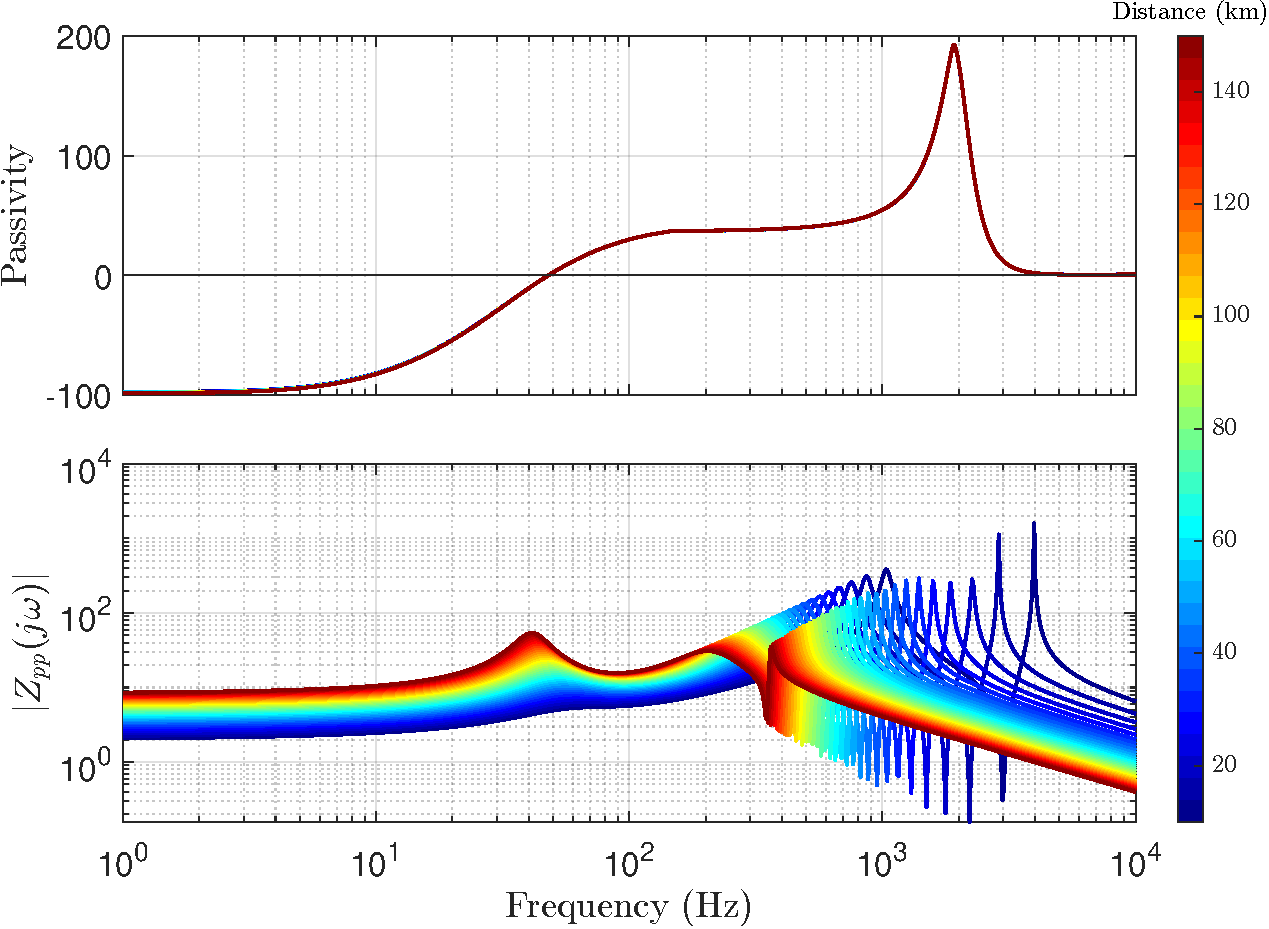
\includegraphics[width=0.8\textwidth]{Figures/vary_cable.pdf}
  \caption{Parameter sweep example (distance sweep).}
\end{figure}

Change \texttt{p\_vary.name} to any field in the \texttt{WF} struct (dot-separated path) and \texttt{p\_vary.val} to your sweep vector.

\subsection{Included tests}
\begin{itemize}
  \item Onshore vs. offshore and GFL vs. GFM
  \item Sweep of transmission distance
  \item Sweep of number of turbines connected
  \item Sweep of grid impedance
  \item Sweep of active and reactive power references
  \item Enabled/disabled voltage feedforward
  \item Sweep of active damping
  \item Sweep of virtual impedance (GFM)
  \item Sweep of droop gains and VSM parameters
\end{itemize}

\section{Useful Functions}
There are several useful functions included to help with analysis and plotting of the results besides the ones directly used for calculating the wind farm impedances. They are:

\begin{itemize}
    \item \texttt{plot\_p\_vary}: Plots the passivity and impedance of either a single impedance or array of impedances as a function of the frequency. The impedances should be a frequency response object, \texttt{frd}. This uses the function \texttt{mimo\_passivity} to calculate the passivity. 
    \item \texttt{mimo\_passivity}: Calculates the equation: $\mathrm{eig}\left[\mathbf{Z}(j\omega)+\mathbf{Z}^H(j\omega)\right]>0$ for a MIMO impedance defined as an \texttt{frd.}
    \item \texttt{setNestedField}: Sets an arbitrary field that may be nested by listing the full field name as a string. This is useful for parameter sweeps. 
\end{itemize}

\end{document}
